% This file was created by matlab2tikz v0.4.7 running on MATLAB 7.14.
% Copyright (c) 2008--2014, Nico Schlömer <nico.schloemer@gmail.com>
% All rights reserved.
% Minimal pgfplots version: 1.3
% 
% The latest updates can be retrieved from
%   http://www.mathworks.com/matlabcentral/fileexchange/22022-matlab2tikz
% where you can also make suggestions and rate matlab2tikz.
% 
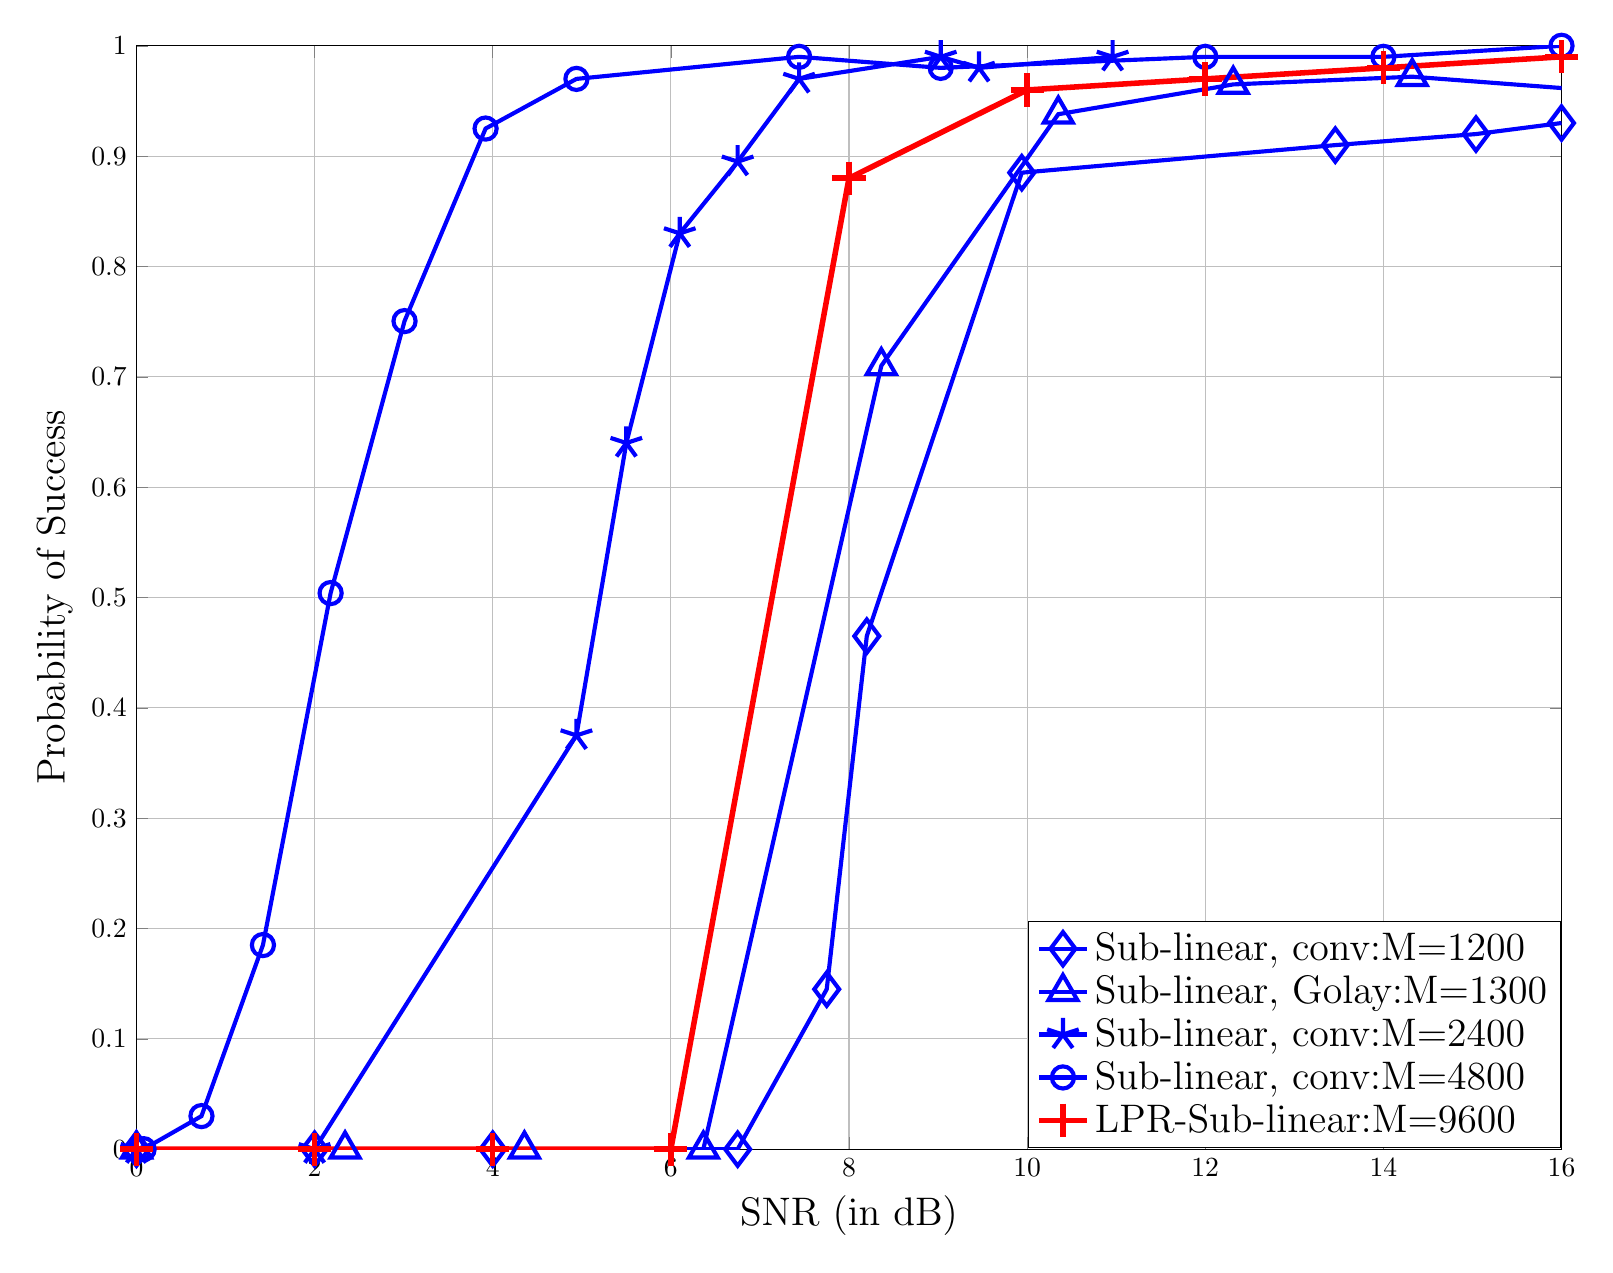
\begin{tikzpicture}

\begin{axis}[%
width=7.12521981627297in,
height=5.51690441819773in,
scale only axis,
xmin=0,
xmax=16,
xmajorgrids,
ymin=0,
ymax=1,
ymajorgrids,
 %xtick = {0,1,2,3,4,5,6,7,8,9,10,11,12,13,14,15,16},
xtick = {0,2,4,6,8,10,12,14,16},
xlabel={\Large{SNR (in dB)}},
ylabel={\Large{Probability of Success}},
legend style={at={(1.0,0.0012)},anchor=south east,draw=black,fill=white,legend cell align=left,font=\Large}
]


%\addplot [color=green,solid,line width=1.5pt,mark size=4.0pt,mark=pentagon,mark options={solid}]
%  table[row sep=crcr]{16	0.95\\
%15.05	0.92\\
%12.12	0.89\\
%9.94	0.875\\
%8.2	0.585\\
%7.81	0.33\\
%7.44	0.115\\
%6.1	0\\
%};
%\addlegendentry{Sub-linear:M=1300};


%Convolutional Code 1/2 rate. No sign row
\addplot [color=blue,solid,line width=1.5pt,mark size=6.0pt,mark=diamond,mark options={solid}]
  table[row sep=crcr]{ 16 0.93\\
  15.04 0.92\\
13.46   0.91\\
9.94   0.8850\\
8.20  0.4650\\
7.75 0.1450\\
6.75 0\\
4 0\\
2  0\\
0	0\\
};
\addlegendentry{Sub-linear, conv:M=1200};

\addplot [color=blue,solid,line width=1.5pt,mark size=6.0pt,mark=triangle,mark options={solid}]
  table[row sep=crcr]{0 0\\
%  2 0\\
%  4 0\\
%  6.1 0.1\\
%  8.01 0.82\\
%  10.043  0.96\\
%  12.0057 0.964\\
%  14 0.97  0.97\\
2.342 0\\
4.356 0\\
6.365 0\\
8.363    0.71\\
10.35    0.938\\
12.314 0.965\\
14.324  0.972\\
 16.28 0.96\\
};
\addlegendentry{Sub-linear, Golay:M=1300};

\addplot [color=blue,solid,line width=1.5pt,mark size=6.0pt,mark=star,mark options={solid}]
  table[row sep=crcr]{0 0\\
  2 0\\
  4.94 0.375\\
  5.50 0.64\\
  6.10 0.83\\
  6.75 0.895\\
  7.44 0.97\\
9.03  0.99\\
  9.46 0.98\\
  10.96 0.99
  13.46 0.985\\
};
\addlegendentry{Sub-linear, conv:M=2400};

\addplot [color=blue,solid,line width=1.5pt,mark size=4.0pt,mark=o,mark options={solid}]
  table[row sep=crcr]{ 16 1\\
  14 0.99\\
  12 0.99\\
  9.03 0.98\\
7.44 0.99
  6.10  0.97\\
  4.94  0.97\\
  3.92  0.925\\
  3.01  0.7505 \\
  2.18  0.504\\
  1.42 0.185\\
  0.73 0.03\\
  0.08 0\\
};
\addlegendentry{Sub-linear, conv:M=4800};

\addplot [color=red,line width=2.0pt,mark size=6.0pt,mark=+,mark options={solid}]
  table[row sep=crcr]{0	0\\
2	0\\
4	0\\
6	0\\
8	0.88\\
10	0.96\\
12	0.97\\
14	0.98\\
16	0.99\\
};
\addlegendentry{LPR-Sub-linear:M=9600};

%\addplot [color=red,dashed,line width=1.5pt,mark size=6.0pt,mark=square,mark options={solid}]
%  table[row sep=crcr]{0	0\\
%2	0\\
%4	0\\
%6	0.005\\
%8	0.08\\
%10	0.215\\
%12	0.43\\
%14	0.58\\
%16	0.65\\
%};
%\addlegendentry{LPR-Near-linear:M=1200};
%
%\addplot [color=red,dashed,line width=1.5pt,mark size=6.0pt,mark=triangle,mark options={solid}]
%  table[row sep=crcr]{0	0\\
%2	0.04\\
%4	0.78\\
%6	0.95\\
%8	0.97\\
%10	1\\
%12	1\\
%14	1\\
%16	1\\
%};
%\addlegendentry{LPR-Near-linear:M=2400};


%\addplot [color=blue,solid,line width=1.5pt,mark size=6.0pt,mark=otimes,mark options={solid}]
%  table[row sep=crcr]{0	0\\
%2.18      0     \\
%3.01 0.0700 \\
%3.92  0.4200 \\
%4.94  0.7400 \\
%6.10  0.9450 \\
%7.44  0.9900 \\
%9       0.999   \\
%12     1.00    \\
%};
%\addlegendentry{BCH-Near-linear:M=2400};


\end{axis}
\end{tikzpicture}%